\documentclass[a4paper,11pt]{article}

% fonts
\usepackage[utf8]{inputenc}
%\usepackage[francais]{babel}

% to get hyphenation on accented words
\usepackage[T1]{fontenc}

% href
\usepackage{hyperref}
\hypersetup{
    colorlinks=true,
    linkcolor=blue,
    filecolor=blue,      
    urlcolor=blue,
    bookmarks=true
}

% quotes
\usepackage{csquotes}

% code highlighting
\usepackage{minted}
\usemintedstyle{pastie}

% asm
\usepackage{amsmath}
\usepackage{amssymb}
\usepackage{amsthm}

% inline code
\usepackage{listings}
\usepackage{xcolor}

% tables
\usepackage{booktabs}

% algorithm
\usepackage[]{algorithm2e}

% for right cases
\newenvironment{rcases}
  {\left.\begin{aligned}}
  {\end{aligned}\right\rbrace}
  
% images
\usepackage{graphicx}
\usepackage{float}

% diagrams
\usepackage{tikz}
\usetikzlibrary{matrix}
\usetikzlibrary{positioning}

% tables
\usepackage{booktabs}

% no identation
\setlength{\parindent}{0pt}

% theorem
\newtheorem{definition}{Definition}
\newtheorem{property}{Property}
\newtheorem{theorem}{Theorem}

% header
\title{How to backdoor Diffie-Hellman, lessons learned from the Socat non-prime prime}
\author{David Wong}
\date{\emph{NCC Group}, \small{February 2016}}

% 
\begin{document}

\maketitle

\renewcommand{\abstractname}{Abstract}
\begin{abstract}
A few months after Juniper's infamous and subtle vulnerability at the end of 2015, A similar fine tuning happened in an open source tool called Socat. Juniper's cryptographic vulnerability was found to have birthed from the change of a simple number later identified as a Dual EC parameter (NSA's backdoored Pseudo-Random Number Generator). Socat's own change of number happened to be in its implementation of the Diffie-Hellman key exchange. This paper aims to introduce the point of view of a malicious commiter who would want to introduce a Nobody-But-Us backdoor in the later public key cryptosystem he has access to.\\
\\
\textbf{Keywords:} Juniper, Socat, NOBUS, backdoor, Dual EC, Diffie-Hellman, Small subgroup attack, Pohlig-Hellman, Factorization, Pollard's p-1 algorithm, ECM\\

\end{abstract}

\section{Introduction}\label{introduction}

Around Christmas 2015, a company named \emph{Juniper} released an \href{https://kb.juniper.net/InfoCenter/index?page=content&id=JSA10713&actp=search}{out of cycle security bulletin}. Two vulnerabilities were being half-disclosed, without much details to help us grasp the seriousness of the situation. Fortunately, at this period of the year many researchers were home with nothing else to do but to try  solving this puzzle. Quickly, by diffing both the patched and vulnerable binaries, the two issues were pinpointed. While one of the vulnerability was a simple super password implemented at a crucial step of the product's authentication, the other vulnerability discovered was a bit more subtle: a value was modified. More accurately, a number was replaced. The introduction of the vulnerability was so trivial that the simple use of the unix commandline tool \mintinline{bash}{strings} was enough to discover the change.

\begin{figure}[H]
\centering
\includegraphics[scale=.6]{screenOS.png}
\caption{The Juniper's Security Bulletin}\label{screenOS}
\end{figure}

Behind that modified number was hiding a \emph{Dual EC} value. Dual EC is a Pseudo-Random Number Generator (PRNG) that is believed to have been backdoored by the NSA \cite{dualEC}. The PRNG's core has the ability to provide a Nobody But Us (NOBUS) trapdoor: a secret passage that can only be accessed by the people holding the secret key. In our case: the elliptic curve discrete logarithm $k$ in the Dual EC equation $Q = [k]P$ (where $P$ and $Q$ are the two elliptic curve points used in the foundation of Dual EC).\\

\begin{figure}[H]
\centering
\includegraphics[width=\textwidth]{screenOS2.png}
\caption{The Juniper's Security Bulletin}\label{screenOS}
\end{figure}

Although the quest to find the Juniper's backdoor and the numerous open questions that arose from that work are a fascinating read by itself \cite{juniper}, it is only the introduction of this work that aims to show how secure and strong cryptographic constructions are a simple and subtle change away from being your own secretive pipe-show.\\

On February the 1st 2016, only a few months after Juniper's debacle, \emph{Socat} \href{http://www.openwall.com/lists/oss-security/2016/02/01/4}{published a security advisory of its own}.

\begin{displayquote}
In the OpenSSL address implementation the hard coded 1024 bit DH p parameter was not prime. The effective cryptographic strength of a key exchange using these parameters was weaker than the one one could get by using a prime p. Moreover, since there is no indication of how these parameters were chosen, the existence of a trapdoor that makes possible for an eavesdropper to recover the shared secret from a key exchange that uses them cannot be ruled out.\\
A new prime modulus p parameter has been generated by Socat developer using OpenSSL dhparam command.\\
In addition the new parameter is 2048 bit long
\end{displayquote}

This is alerting. In the same vein of Juniper's problem, a single number was changed. But Socat's problems root deeper. A year before that suspicious 1024 bit Diffie-Hellman (DH) value was introduced, the free software would have served its TLS connection using a 512 bit DH modulus. The problem with such small DH parameters is already well known \cite{logjam}, but the problems of implementing DH securely are unfortunately rarely well understood. The defense approach is told in several RFCs \cite{rfc2631} \cite{rfc2785}, but no paper so far take the point of view of the attacker.\\

In section 2, we will first discard some possible mistakes that the troublemaker could have made. In section 3 we will introduce the different attacks available on DH, from small subgroup attacks to Pohlig Hellman's algorithm. We will start by explaining how to implement a NOBUS backdoor in Diffie-Hellman in section 4, and we will follow with the bulk of our contribution in section 5: that is the different methods to achieve that goal. In section 6 we will see what's wrong with the previous methods, and use what we learned from that to try to reverse Socat's 1024 bit DH modulus. Informationally, we will test the security of the new 2048 bit DH modulus of Socat in section 7, and follow by brief explanations on how to secure a DH implementation. Eventually we will wrap it all in section 9.

\section{Human error}\label{mistake}

Before shouting from the rooftops the words "backdoor", let's take a step back and imagine what could have gone wrong. First, it is possible that \href{http://repo.or.cz/socat.git/commitdiff/281d1bd6515c2f0f8984fc168fb3d3b91c20bdc0}{the poor man who suggested the change} (back then an \emph{Oracle} employee) had no idea that the DH modulus should be a prime. In fact, Diffie-Hellman works well enough with composite modulus (but keep in mind that it has its share of problems, and we will see later why). Also, what if he did generated a prime but got lost afterwards?\\

Throughout TLS \cite{tls12}, and in Socat's case throughout OpenSSL, the use of \emph{big endianness} is enforced for long numbers formatting. That is: you read a byte string from left to right to convert it to a number. This can make the process of converting from and to numbers a confusing task.

\begin{figure}[H]
\begin{minted}[breaklines,frame=single]{c}
static unsigned char dh1024_p[] = {
   0xCC, 0x17, 0xF2, 0xDC, 0x96, 0xDF, 0x59, 0xA4, 0x46, 0xC5, 0x3E, 0x0E, 
   0xB8, 0x26, 0x55, 0x0C, 0xE3, 0x88, 0xC1, 0xCE, 0xA7, 0xBC, 0xB3, 0xBF, 
   0x16, 0x94, 0xD8, 0xA9, 0x45, 0xA2, 0xCE, 0xA9, 0x5B, 0x22, 0x25, 0x5F, 
   0x92, 0x59, 0x94, 0x1C, 0x22, 0xBF, 0xCB, 0xC8, 0xC8, 0x57, 0xCB, 0xBF, 
   0xBC, 0x0E, 0xE8, 0x40, 0xF9, 0x87, 0x03, 0xBF, 0x60, 0x9B, 0x08, 0xC6, 
   0x8E, 0x99, 0xC6, 0x05, 0xFC, 0x00, 0xD6, 0x6D, 0x90, 0xA8, 0xF5, 0xF8, 
   0xD3, 0x8D, 0x43, 0xC8, 0x8F, 0x7A, 0xBD, 0xBB, 0x28, 0xAC, 0x04, 0x69, 
   0x4A, 0x0B, 0x86, 0x73, 0x37, 0xF0, 0x6D, 0x4F, 0x04, 0xF6, 0xF5, 0xAF, 
   0xBF, 0xAB, 0x8E, 0xCE, 0x75, 0x53, 0x4D, 0x7F, 0x7D, 0x17, 0x78, 0x0E, 
   0x12, 0x46, 0x4A, 0xAF, 0x95, 0x99, 0xEF, 0xBC, 0xA6, 0xC5, 0x41, 0x77, 
   0x43, 0x7A, 0xB9, 0xEC, 0x8E, 0x07, 0x3C, 0x6D, 
};
\end{minted}
\caption{Socat's 1024 bit DH non-prime prime}
\label{fig:cert}
\end{figure}

Passed to OpenSSL, this big number is read from left to right as the long hexstring. Passed through a primality test this is indeed a composite number.

\begin{figure}[H]
\centering
\includegraphics[width=\textwidth]{prime1.png}
\end{figure}

A natural question we could ask ourselves is that maybe the rogue commiter could have reversed the hexstring? Testing for that yielded a composite number as well.

\begin{figure}[H]
\centering
\includegraphics[width=\textwidth]{prime2.png}
\end{figure}

What if everything was reversed? Even inside the byte

\begin{figure}[H]
\centering
\includegraphics[width=\textwidth]{prime3.png}
\end{figure}

Another one, is that maybe the prime number was too long and thus truncated to 1024 bit (since the program was asking for a 1024 bit number). Indeed, the following number is a prime:

\begin{figure}[H]
\centering
\includegraphics[width=\textwidth]{prime4.png}
\end{figure}

It might comes as a shock to the non-enlightened, but we usually do not take the time to generate real primes, or what we more generally call \emph{provable} primes. Efficient provable tests like ECPP or AKS \cite{ecpp} do exists, but the accuracy and the speed of \emph{probable} tests (tests that either tell you if a number is probably a prime, or definitely not a prime) are good enough that any margin of error is negligible.

Examples of probable tests are given in appendix C.3 of the  \href{http://csrc.nist.gov/publications/fips/fips186-3/fips_186-3.pdf}{FIPS 186 document}. Most implementations will use the \emph{Miller-Rabin} test with a variable amount of iteration according to the degree of certainty they want to achieve.

For example in \href{https://www.openssl.org/docs/manmaster/crypto/BN_generate_prime.html}{Openssl's \mintinline{c}{BN_is_prime_fasttest_ex()} function}, the number of iteration is chosen such that the risk of yielding a false positive (a non-prime prime) is of at most $1/2^{80}$. To understand what this means in practice: it is as likely to happen as being hit by a meteorite while winning the Powerball. Here's a quote from the Structure and Interpretation of Computer Programs book \cite{sicp}:

\begin{displayquote}
Numbers that fool the Fermat test are called Carmichael numbers, and little is known about them other than that they are extremely rare. There are 255 Carmichael numbers below 100,000,000. The smallest few are 561, 1105, 1729, 2465, 2821, and 6601. In testing primality of very large numbers chosen at random, the chance of stumbling upon a value that fools the Fermat test is less than the chance that cosmic radiation cosmic radiation will cause the computer to make an error in carrying out a "correct" algorithm. Considering an algorithm to be inadequate for the first reason but not for the second illustrates the difference between mathematics and engineering.
\end{displayquote}

This is to say: the Oracle developer probably didn't intend to generate a prime.

\section{Attacks on Diffie-Hellman}

Diffie-Hellman has two unfamous related attacks, \emph{Pohlig-Hellman} and \emph{Small subgroups attacks}, that work well when the modulus is \emph{weak}. That is: the group it creates has an composite order whose factor are too small. while DH can work in any kind of integer group, there are methods to make it more secure, for example by choosing a \emph{safe prime} as the modulus.

A safe prime $p$ is a special prime of the form $p = 2q + 1$ where $q$ is prime\footnote{the prime $q$ is called a \emph{Sophie Germain prime} in this case}. This allows the order of the group it creates to be $p - 1 = 2q$, which main factor is big enough for the following attacks not to work.

\subsection{The Chinese Remainder Theorem}

Along LLL, SAT solvers, the General Number Field Sieve, Pollard's Rho and the Euclidian algorithm, the \emph{Chinese Remainder Theorem} (CRT) is one of the magic tool of a cryptanalyst.

This tool sometimes used for the good (RSA-CRT\footnote{ Shinde, Fadewar \href{http://www.techscience.com/doi/10.3970/icces.2008.005.255.pdf}{Faster RSA Algorithm for Decryption Using Chinese
Remainder Theorem}}\cite{fasterRSA} is a construction where CRT is used to speed up RSA decryption) is also often used for the bad. But first let's see how it works:

\begin{theorem}
Suppose $m = \prod^{k} m_i$ with $m_1, \cdots, n_k$ pairwise co-prime.\\

For any $(a_1, \cdots, a_k)$ there exists a $x$ such that:\\

\begin{cases}
x= a_1 \pmod{m_1}\\
\vdots\\
x= a_k \pmod{m_k}\\
\end{cases}\\

And there exist a unique solution for $x \pmod{m}$
\end{theorem}

There is a simple proof to that theorem which we will use to later reconstruct a $x \pmod{m}$ in the attack (note that I called the modulus $m$ so that you don't get any ideas that we will later use CRT with a DH modulus). Here goes the proof:

\begin{proof}
\begin{equation*}
x = \sum^{k} a_i * (\prod_{j \neq i} m_j (m_j^{-1} \pmod{m_i}))  \pmod{m}
\end{equation*}
\end{proof}\\

At first, it might be kind of hard to grasp where that formula is coming from. But let me explain by starting with only two equations. Keep in mind that we want to find the value of $x$ modulo $m = m_1 m_2$

\[
\begin{rcases}
x = a_1 \pmod{m_1}\\
x = a_2 \pmod{m_2}
\end{rcases}
\implies x = \text{ ?} \pmod{m}
\]\\

How can we start building the value of $x$?
\begin{multline}
\begin{aligned}
&\text{If } x = a_1  m_2\pmod{m} \text{,}\\
&\text{then }
\begin{cases}
x = \boldsymbol{a_1} m_2 \pmod{m_1}\\
x = \boldsymbol{0} \pmod{m_2}\\
\end{cases}\\
\end{aligned}
\end{multline}

Quite not what we want, but we are getting there. Let's add to it:
\begin{multline}
\begin{aligned}
&\text{If } x = a_1  m_2  (m_2^{-1} \pmod{m_1}) \pmod{m}\\
&\text{then } \begin{cases}
x = a_1 m_2 (m_2^{-1} \pmod{m_1}) = \boldsymbol{a_1} \pmod{m_1}\\
x = 0 \pmod{m_2}\\
\end{cases}\\
&\text{with } $m_2{-1} \pmod{m_1}$ \text{the inverse of} $m_2$ \text{modulo} $m_1$\text{.}
\end{aligned}
\end{multline}

That's almost what we want! Half of what we want actually. We just need to do the same thing for the other side of the equation, and we have:\\

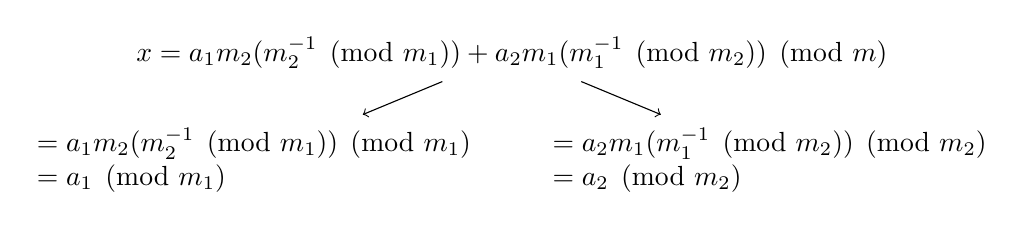
\begin{tikzpicture}[scale=.55]
% main formula
\node (main) {$x = a_1 m_2 (m_2^{-1} \pmod{m_1}) + a_2 m_1 (m_1^{-1} \pmod{m_2}) \pmod{m}$};
% other formulas
\node (formula1) [below left=.5cm and -4.5cm of main, align=left] {$= a_1 m_2 (m_2^{-1} \pmod{m_1}) \pmod{m_1}$\\$= a_1 \pmod{m_1}$};
\node (formula2) [below right=.5cm and -4.5cm of main, align=left] {$= a_2 m_1 (m_1^{-1} \pmod{m_2}) \pmod{m_2}$\\$= a_2 \pmod{m_2}$};
% arrows
\draw [->, shorten <=3pt, shorten >=3pt] (main) -- (formula1);
\draw [->, shorten <=3pt, shorten >=3pt] (main) -- (formula2);
\end{tikzpicture}

Everything works as we wanted! Now you should understand better how we came up with that general formula in the proof.

\subsection{Pohlig Hellman}

Now what if we could use the Chinese Remainder Theorem to attack Diffie-Hellman? That must what have been thinking Stephen Pohlig and Martin Hellman when they designed their algorithm.\\

One way of attacking Diffie-Hellman is to compute the discrete-logarithm $x$ of one of the peer's public keys $y = g^{x}$ modulo the modulus $n$ (here both $g$ and $n$ are fixed parameters). Let's take a closer look at the private exponent $x$. Euler's Totient Theorem states that:

\begin{theorem}
If $n$ and $g$ are coprime positive integers, then
\[ g^{\varphi(n)} = 1 \pmod{n} \]
\end{theorem}

This tells us that the private exponent $x$ can be written modulo $\varphi(n) = \prod p_i^{k_i}$, the order of the group.\\

So what if we could reduce the problem of finding $x \pmod{\varphi(n)}$ by finding $x \pmod{p_i^{k_i}$ for each $i$ and then easily retrieving it modulo $\varphi(n)$ with our new CRT tool? In fact a theorem says it is possible:

\begin{theorem}
Let $n$ be a composite integer. The discrete logarithm problem in $\mathbb{Z}^*_n$ polytime reduces to the combination of the integer factorization problem and the discrete logarithm problem in $\mathbb{Z}^*_p$ for each prime factor $p$ of $n$.
\end{theorem}

And the proof of the theorem is our attack: Pohlig Hellman. It goes as follow:

\begin{enumerate}
    \item Determine the prime factorization of the order of the group
        $$\varphi(n) = \prod p_i^{k_i} $$
    \item Determine the value of $x$ modulo $p_i^{k_i}$ for each $i$
    \item Recompute $x \pmod{\varphi(n)}$ with the Chinese Remainder Theorem
\end{enumerate}

The main idea of Pohlig-Hellman's method is in how do we determine the value of $x$ modulo each $p_i^{k_i}$. One way of doing it is to try to reduce our public key to the subgroup we're looking at by computing:

$$y^{\varphi(n)/p_i^{k_i}} \pmod{n}$$

Computing the discrete logarithm of that value, we get $x \pmod{p_i^{k_i}}$. This works because of the following observation:
$$ x = x_1 + p_i^{k_i} x_2 $$

\begin{align*}
    y^{\frac{\varphi(n)}{p_i^{k_i}}} &= (g^{x})^{\frac{\varphi(n)}{p_i^{k_i}}} \pmod{n}\\
    &= g^{\frac{(x) \varphi(n)}{p_i^{k_i}}} \pmod{n}\\
    &= g^{\frac{(x_1 + p_i^{k_i} x_2) \varphi(n)}{p_i^{k_i}}} \pmod{n}\\
    &= g^{\frac{x_1 \varphi(n)}{p_i^{k_i}}} g^{x_2 \varphi(n)} \pmod{n}\\
    &= g^{\frac{x_1 \varphi(n)}{p_i^{k_i}}} \pmod{n}\\
\end{align*}

note: in theory we can't reduce if we're in a smaller group, we can't "escape", we can only go in small subgroups

note2: running time of pollard's rho is approximately $\mathbb{O}(\sqrt{n})$ => running time of Pohlig Hellman in total is $\mathbb{O}(\sqrt{p})$ where $p$ is the largest prime factor of $n$.

\subsection{Small subgroup attacks}

> Static Diffie-Hellman keys are vulnerable to a small subgroup attack

The previous attack is "impractical" because DH is usually used as DHE (ephemeral keys). And since it is an active attack where we need to do several "handshake" (is this called a handshake?)

Pohlig Hellman is a passive attack, and spying on only one conversation allows you to decrypt the rest

---

* There exist an easier way than Pohlig Hellman, instead of computing the thing we just send the right generator right away
* but it doesn't work in dhe
* most people use dhe, not dh

http://citeseerx.ist.psu.edu/viewdoc/download?rep=rep1&type=pdf&doi=10.1.1.44.5296

(d'un autre lien)> The small subgroup attack was first pointed out by Vanstone[26]; see also van Oorschot and Wiener [36], Anderson and Vaudenay [1], and Lim and Lee [22].

if the order is a composite of small subgroups

why not getting the discrete log in different subgroup and recombine it with CRT? That sounds easier that getting the discrete log in the whole group


\section{How to implement a backdoor in DH}

\subsection{Nobody But Us}

we could use what we saw previously as such:

generate a prime such that the order of the generated group is p-1 a composites where the dlog is "do-able" in its subgroups. We don't need smooth. Doable is defined by your the computation power of the backdoor creator

But then anyone is able to get the order of the group (p-1) and can then factor that order. [[dlog in k bits is factor in 2 kbits no? Check complexities of these]]

It is believed by some that the NSA is a bit more classy than that and would create what we call "Nobody But Us" types of backdoor. That is nobody can reverse them. This was the case of Dual EC (although Dual EC suffered from slowness and bit biases even without the backdoor)

A good way of doing that is to use a non-prime modulus, this way the order would be $\varphi(n)$ which is not p-1 anymore (give the formula)

From the theorem Polhig Helman (ref) this would put a barrier of entry to the backdoor: if you are not the one who generated the backdoor values, you would first have to factor the modulus in order to compute the order in order to perform the Pohlig Hellman attack.

\section{Methods to create a backdoor} title)}

\subsection{method 1}

creating a backdoor method 1: p = p_1 p_2 where p_i - 1 smooth

\subsection{Method 2}

\subsection{Method 3}

\section{Methods to reverse the backdoor}

\subsection{trial division}

we found 271 and 13,597

\subsection{pollard p-1}

such a construction as method1 allows for p-1 pollard to work.

\subsubsection{explanation}

explanation of pollard p-1

\subsubsection{results}

We tried it on a proof of concept and: RESULT

we then tried it on socat's dh1024_p and: RESULT

\subsection{ECM}

not tied to the modulus size, but tied to the smallest factor

on our proof of concet: RESULT

on socat's dh1024_p: RESULT

\section{Estimations}

\subsection{Past records of factorization}

list of integer factorization: http://www.loria.fr/~zimmerma/records/factor.html
list of ECM factorization: http://www.loria.fr/~zimmerma/records/top50.html

> 73-digit prime found in 2010 by J. Bos, T. Kleinjung, A. Lenstra and P. Montgomery.
 
http://homes.cerias.purdue.edu/~ssw/cun/press/tech.html
>  On August 2, 2012, Wagstaff found the 75-digit factor
336842026814486816413712532665671525518487238461533945786937785048474675329
of 11304+1.
> Ten days later, on August 12, 2012, he found the 79-digit factor
2302872188505279576573535015926441913945044975483579529517513795897664211127797
of 11306+1. 

http://mersenneforum.org/showpost.php?p=352425&postcount=5
http://mersenneforum.org/showpost.php?p=352452&postcount=11
> late 2013, Ryan Propper reported using GMP-ECM 6.4.3 + GMP 5.1.0 to find a 274-bit factor from the 787-bit composite (7337+1)/8/101020140256422276570987002251440602782290400709 product of two unknown primes, on a commodity CPU using less than 6GB of RAM. He further reports that was a 10-day effort on Stanford's University cluster, and the factorization was found after 5000 curves.

http://crypto.stackexchange.com/questions/15823/multiple-prime-rsa-how-many-primes-can-i-use-for-a-2048-bit-modulus
> odds of finding that factorization so fast where 1/400; "this was quite the lucky find" is an understatement

\subsection{Past records of discrete logarithm in prime group}

> The discrete logarithm problem is considered to be computationally intractable. That is, no efficient classical algorithm is known for computing discrete logarithms in general.

so we can't dlog anything like that. We need some small subgroups

https://en.wikipedia.org/wiki/Discrete_logarithm_records

> On 18 June 2005, Antoine Joux and Reynald Lercier announced the computation of a discrete logarithm modulo a 130-digit (431-bit) strong prime in three weeks, using a 1.15 GHz 16-processor HP AlphaServer GS1280 computer and a number field sieve algorithm.

> On 5 February 2007 this was superseded by the announcement by Thorsten Kleinjung of the computation of a discrete logarithm modulo a 160-digit (530-bit) safe prime, again using the number field sieve. Most of the computation was done using idle time on various PCs and on a parallel computing cluster.

> On 11 June 2014, Cyril Bouvier, Pierrick Gaudry, Laurent Imbert, Hamza Jeljeli and Emmanuel Thomé announced the computation of a discrete logarithm modulo a 180 digit (596-bit) safe prime using the number field sieve algorithm.

\section{The new modulus and how to secure a DH implementation}

new modulus=it was done p = 2q + 1 with q prime


- if the p = 2q + 1 is not done like that, there is a RFC that tells you how to secure such DH (safe prime, or is it Sophie Germaine prime? Or strong prime?)

- openssl dhparam

- also some people believe generation of prime is too difficult and that it shouldn't be possible (rfc with predefined dh groups). But then weakdh (or was it logjam rather), everybody used the same hardcoded dh prime, everybody could have/got owned

- verification of public key (but there is a patent on that? According to the diffie-hellman RFC)

- generation of safe prime

\subsection{Uniform Distribution}

How does a non-malicious, mistakenly, badly generated composite modulus, should be distributed (and we will later come back to this):

From \href{http://cacr.uwaterloo.ca/hac/about/chap3.pdf}{Handbook of Applied Cryptography fact 3.7}:

\begin{definition}
    Let $n$ be chosen uniformly at random form the interval $[1, x]$.
    \begin{enumerate}
        \item if $1/2 \leq \alpha \leq 1$, then the probability that the largest prime factor of $n$ is $\leq x^{\alpha}$ is approximately $1+ ln(\alpha)$. Thus, for example, the probability than $n$ has a prime factor $> \sqrt(x)$ is $ln(2) \approx 0.69$
        \item The probability that the second-largest prime factor of $n$ is $\leq x^{0.2117}$ is about $1/2$. 
        \item The expected total number of prime factors of $n$ is $ln ln x + \mathcal{O}(1)$. (If $n = \prod p_i^{e_i}$, the total number of prime factors of n is $\sum e_i$.)
    \end{enumerate} 
\end{definition}

And since it might be easier to visualize this with numbers:

\begin{enumerate}
    \item socat's 1024 bit composite modulus $n$ probability to have a prime factor greater than 512 bits is $\approx 0.69$.
    \item the probability that the second-largest prime factor of $n$ is smaller than 217 bits is $1/2$.
    \item The total number of prime factor of $n$ is expected to be $7$.
\end{enumerate}


\subsection{Our results}

CONCLUSION: we shouldn't be able to find anything if the distribution is uniform

CONCLUSION: from theorem in Pohlig Hellman that DH -> factorization+DLOG:
* we need hard factorization
* we need easy dlog
^ to make the backdoor working

CONCLUSION: 
* if the groups are small enough we can find them and discrete log is easy (not  NOBUS backdoor)
* if the groups are too big we can't find them but discrete log can't be computed (not a backdoor)
* if the groups are in range(X, Y) we can't find them, and only a big player can compute the DLOG (NSA) which makes sense (NOBUS backdoor)

TODO:
* we will only optimize p-1 for the first case (not NOBUS backdoor)
* same for ECM

from mersennewiki:
> ECM on 70-digit factors is almost impossible with current hardware

we ran ECM and pollard p-1 on two machines [descript of machine] with no results
the number we are trying to find is a 302 digits composite (C302)

271 and 13597 was found after trial division

we tested if the generator $g=2$ was confined to one of the subgroup of order 270 or 13596: nope. (g^270 mod n != 1)

CONCLUSION:
1) if we find something => might not be a NOBUS?
2) if we don't find anything => might be NOBUS, might just be uniform distrib
hard to conclude... revise this

\section{Conclusion}

- implementing DH correctly is not that hard
- easy to backdoor
- is it really a backdoor? Since we can't factor it... maybe not (maybe give estimations to factor it, and to use the backdoor if it is indeed a backdoor with such big factors)
- people need to verify open source
- people are going away from DHE and to ECDHE ( https://weakdh.org/sysadmin.html )
\newpage

\section*{Acknowledgements}


\newpage

\begin{thebibliography}{1}

\bibitem{dualEC} Bernstein, Lange and Niederhagen \href{https://eprint.iacr.org/2015/767.pdf}{Dual EC: A Standardized Back Door}

\bibitem{juniper} Juniper {\em Juniper}

\bibitem{logjam} Adrian, Bhargavan, Durumeric, Gaudry, Green, Halderman, Heninger, Springall, Thomé, Valenta,  VanderSloot, Wustrow, Zanella-Béguelin, Zimmermann \href{https://weakdh.org/imperfect-forward-secrecy-ccs15.pdf}{Imperfect Forward Secrecy: How Diffie-Hellman Fails in Practice}

\bibitem{rfc2631} RFC 2631: \href{https://tools.ietf.org/html/rfc2631}{Diffie-Hellman Key Agreement Method}

\bibitem{rfc2785} RFC 2785: \href{https://tools.ietf.org/html/rfc2785}{Methods for Avoiding the "Small-Subgroup" Attacks on the Diffie-Hellman Key Agreement Method for S/MIME}

\bibitem{ecpp} Frank Li \href{http://theory.stanford.edu/~dfreeman/cs259c-f11/finalpapers/primalityproving.pdf}{An Overview of Elliptic Curve Primality Proving}

\bibitem{sicp} Abelson, Sussman, Sussman \href{https://mitpress.mit.edu/sicp/chapter1/footnode.html#2413}{Structure and Interpretation of Computer Programs}

\bibitem{tls12} RFC 5246: \href{https://www.ietf.org/rfc/rfc5246.txt}{The Transport Layer Security (TLS) Protocol Version 1.2}

\bibitem{fasterRSA} Shinde, Fadewar \href{http://www.techscience.com/doi/10.3970/icces.2008.005.255.pdf}{Faster RSA Algorithm for Decryption Using Chinese
Remainder Theorem}

\end{thebibliography}

\end{document}